% !TEX program = pdflatex
% ============================================================
% Execution-Aware Portfolio RL (journal-style single-file manuscript)
% Single-file LaTeX (no external .bib required)
% Author: Kim Geum-Young
% ============================================================

\documentclass[10pt,twocolumn]{article}
\raggedbottom

% ---------- Page / Layout ----------
\usepackage[a4paper,margin=18mm]{geometry}
\usepackage{times}
\usepackage{microtype}

% ---------- Math / Theorems ----------
\usepackage{amsmath,amssymb,amsthm}
\newtheorem{proposition}{Proposition}
\newtheorem{corollary}{Corollary}
\newtheorem{remark}{Remark}

% ---------- Figures / Tables ----------
\usepackage{graphicx}
\usepackage{booktabs}
\usepackage{multirow}
\usepackage{array}
\usepackage{caption}
\usepackage{subcaption}
\usepackage{float}        % for [H]
\usepackage{dblfloatfix}  % improve placement of figure* / table* in twocolumn
\usepackage[section]{placeins}
\setlength{\textfloatsep}{8pt plus 1pt minus 2pt}
\setlength{\dbltextfloatsep}{8pt plus 1pt minus 2pt}
\setlength{\floatsep}{8pt plus 1pt minus 2pt}
\setlength{\intextsep}{8pt plus 1pt minus 2pt}

% ---------- Links ----------
\usepackage[hidelinks]{hyperref}

% ---------- Lists / Colors ----------
\usepackage{enumitem}
\usepackage{xcolor}

% ---------- Misc ----------
\usepackage{url}
\usepackage{authblk}

% ---------- Custom Macros ----------
\newcommand{\wexec}{w^{\mathrm{exec}}}
\newcommand{\wtgt}{w^{\mathrm{tgt}}}
\newcommand{\TOexec}{\mathrm{TO}^{\mathrm{exec}}}
\newcommand{\TOtgt}{\mathrm{TO}^{\mathrm{tgt}}}
\newcommand{\kappaTC}{\kappa}
\newcommand{\R}{\mathbb{R}}
\newcommand{\E}{\mathbb{E}}
\newcommand{\normone}[1]{\left\lVert #1 \right\rVert_1}
\newcommand{\normtwo}[1]{\left\lVert #1 \right\rVert_2}
\newcommand{\DeltaN}{\Delta^N}

% ---------- Title ----------
\title{\vspace{-6mm}
\textbf{Execution-Aware Portfolio Reinforcement Learning via Proximal Execution Control}\\
\vspace{-1mm}
\large Separating Target and Executed Portfolios for Cost-Aligned Evaluation and Execution Stabilization
\vspace{-3mm}
}
\author[1]{Kim Geum-Young}
\affil[1]{Chungbuk National University, Department of Software Engineering}
\date{}

\begin{document}

% ============================================================
% Title + Abstract across both columns (more journal-like)
% ============================================================
\twocolumn[{%
\maketitle
\vspace{-4mm}
\begin{abstract}
\vspace{-1mm}
Most portfolio reinforcement learning (RL) formulations implicitly assume that the portfolio weights output by the policy are immediately executed. Under transaction costs, this conflation misaligns cost accounting and obscures the executed holding path. We formalize a two-stage decomposition: the policy outputs a target portfolio $\wtgt_t$, while a proximal execution controller outputs an executed portfolio $\wexec_t$ via a closed-form update with timescale $\eta_t\in(0,1]$. Costs are charged on executed turnover, not target turnover, so evaluation follows the executed path.
We study this formulation in a deliberately narrow frozen-policy protocol: one control model over a fixed 27-name large-cap U.S. equity snapshot is trained once on 2010--2021, the same trained policy is reused in every empirical arm, and only the execution mapping changes across a fixed $\eta$ grid scored on validation 2022--2023 before final evaluation on 2024--2025. On the canonical split, the locked validation rule selects $\eta=0.5$. On the held-out window, this selected interior operating point reduces median executed turnover from $0.02200$ to $0.01095$ and improves paired median net Sharpe by $+0.0105$ at $\kappa=5\times10^{-4}$ and $+0.0213$ at $\kappa=10^{-3}$ relative to immediate execution, with $10/10$ seed wins in both positive-cost regimes; at $\kappa=0$, the evidence is negligible. Across rolling windows, conservative selected-point transfer is window-sensitive, but the positive-cost held-out frontier remains interior. On a denser canonical friction grid up to $\kappa=2\times10^{-3}$, the best interior held-out gain increases monotonically with friction. These gains are explained by lower realized turnover and lower realized cost, not by improved gross Sharpe. Our claim is therefore narrow: under a fixed learned trading policy, cost-aligned execution control matters under frictions.
\end{abstract}

\vspace{-2mm}
\noindent\textbf{Keywords:} portfolio RL, transaction costs, execution, turnover, proximal control, reproducible backtesting
\vspace{1mm}
\hrule
\vspace{2mm}
}]

% ============================================================
\section{Introduction}
Portfolio RL has gained attention for optimizing dynamic allocations under complex objectives. However, many formulations implicitly assume that the action produced by the agent (portfolio weights) is executed immediately and exactly. In realistic trading---and even in cost-free simulations where policies can over-react and over-trade---the \emph{target} portfolio and the \emph{executed} portfolio are distinct objects:
\begin{itemize}[leftmargin=*,itemsep=1pt]
\item \textbf{Target portfolio} $\wtgt_t$: the policy output at decision time $t$.
\item \textbf{Executed portfolio} $\wexec_t$: the portfolio actually held over the next return interval and used for cost accounting.
\end{itemize}

\paragraph{Terminology convention.}
Throughout the paper, \emph{target portfolio} refers to the policy output $\wtgt_t$, \emph{executed portfolio} refers to the portfolio actually held over the next return interval $\wexec_t$, \emph{immediate-execution baseline} refers to the $\eta=1.0$ comparison arm, \emph{validation-selected operating point} refers to the operating point chosen on the validation window (here $\eta=0.5$), and \emph{net Sharpe} refers to the annualized Sharpe ratio computed from executed net linear returns. The code label \texttt{sharpe\_net\_lin} is simply the implementation name for this same net-Sharpe quantity.

\paragraph{Why this is not ``just smoothing''.}
Execution-aware modeling changes the realized self-financing path, not just the smoothness of an action sequence. If execution is slower than target updates, charging costs on target turnover implicitly rescales the effective cost by $1/\eta_t$ (Proposition~\ref{prop:cost_misalignment}), creating a biased learning signal and misleading evaluation. Moreover, the execution mapping is a proximal step (Proposition~\ref{prop:prox}), equivalent to a low-pass filter on the target trajectory, which stabilizes the \emph{realized trading path} rather than merely penalizing weights directly.

\paragraph{Contributions.}
\begin{enumerate}[leftmargin=*,itemsep=2pt]
\item \textbf{Two-stage decomposition and cost-aligned accounting.} We separate target $\wtgt$ and executed $\wexec$ portfolios, and we define all \emph{core} rewards and performance metrics using $\wexec$ only.
\item \textbf{Execution mapping and accounting implications.} We specify a closed-form execution update parameterized by timescale $\eta_t$ and summarize its basic properties: proximal interpretation, executed-turnover scaling, tracking-error monotonicity, anchor behavior, and target-cost misalignment.
\item \textbf{Frozen-policy validation-first evidence.} Using paired-seed evaluation on a reproducible fixed 27-name large-cap U.S. equity snapshot, we isolate the effect of execution by holding the same learned control policy fixed across all arms, varying only the execution mapping, selecting $\eta$ on validation only, and reserving the test window for held-out evaluation. On the canonical split this produces a validation-selected interior operating point $\eta=0.5$ whose positive-cost held-out benefit is strong; across rolling windows, the positive-cost frontier itself is more robust than the transfer of any single conservative selected point.
\item \textbf{Mechanistic friction-sensitivity diagnostics.} We show that the positive-cost gains are explained primarily by lower realized turnover and lower realized cost rather than by gross-return improvement, and that the same interior frontier becomes more consequential as $\kappa$ increases on a denser canonical friction grid.
\end{enumerate}
This empirical scope is intentionally narrow. Every main empirical result in this paper compares the same trained policy under different fixed execution mappings; no main result is obtained by retraining a different policy under an alternative environment. The paper therefore asks a specific question: under a frozen learned policy, does cost-aligned execution control create an interior positive-cost execution frontier, and are its gains explained primarily by lower realized turnover and lower realized cost rather than by gross-alpha improvement? Correspondingly, the paper does \emph{not} claim retraining superiority, universally transferable selected operating points across windows, broad dominance over classical portfolio strategies, or deployment-grade point-in-time backtest realism. The rolling-window diagnostic further sharpens that scope: the positive-cost execution frontier itself is more stable under rolling windows than the transfer of any single conservative validation-selected operating point. This distinction is also the core gap relative to prior formulations that attach turnover penalties directly to actions while treating actions and holdings as the same object.

% ============================================================
\section{Background and Related Work}
Classical portfolio theory studies dynamic allocation under risk/return trade-offs and frictions \cite{markowitz1952,merton1973}. In friction-aware portfolio optimization, transaction costs are modeled explicitly in both single-period and multi-period allocation problems \cite{lobo2007,garleanu2013}. In particular, dynamic trading with costs naturally separates the currently held portfolio from a moving target portfolio and often leads to partial adjustment or no-trade regions around that target \cite{garleanu2013}. This distinction is even more explicit in optimal-execution models, which trade gradually from a current inventory toward a desired terminal position while balancing execution cost and risk \cite{bertsimas1998,almgren2000}. These literatures motivate our emphasis on the executed portfolio and executed turnover as accounting objects rather than as afterthought diagnostics.

Portfolio RL and deep portfolio management typically make a different interface choice: the policy outputs portfolio weights and the environment treats those weights as the portfolio that is immediately held or rebalanced to \cite{moody1998,jiang2017,ye2020}. Even when transaction costs are included, the agent action and the executed portfolio are often coupled at the same step, so action turnover becomes a proxy for executed trading turnover. Related sequential-allocation work outside RL also studies turnover-aware portfolio updates under trading frictions \cite{li2014}. Recent portfolio-RL variants add auxiliary state prediction, reward shaping, or smoothing penalties to improve robustness and generalization \cite{ye2020,lien2023}. These are valuable advances, but they usually improve representation quality or training stability inside a direct-action portfolio interface rather than separating target and executed holdings as first-class accounting objects.

There is also a broader continuous-control literature on smoothing and regularizing RL policies. Smoothness-inducing policy regularization and action-smoothing methods have been used to improve robustness, stability, and control quality \cite{shen2020,mysore2021}. RL has also been applied directly to trade execution rather than portfolio-weight selection \cite{nevmyvaka2006}. Our execution controller is related in spirit to both strands, but the empirical question here is narrower. The present paper is not primarily about making the policy output look smoother, and it is not a retraining paper about a different RL design. It is about separating target-portfolio decisions from the executed portfolio so that trading costs, net returns, and primary evaluation are attached to the realized executed path under a frozen learned policy.

Our focus is therefore narrower and more specific than a general claim about architecture design. Prior work often treats turnover penalties as part of action regularization, while the present paper treats executed turnover as the quantity that should drive cost accounting and primary evaluation. The resulting contribution is a cost-aligned execution formulation and a frozen-policy empirical study that isolates the execution frontier created by that distinction.

% ============================================================
\section{Problem Setup and Timing (Anti-Lookahead)}
\label{sec:setup}
We consider $N$ risky assets. Let $p_t\in\R^N$ be adjusted close prices and define single-period arithmetic returns over interval $(t,t{+}1]$ by
\[
r_{t+1} \triangleq \frac{p_{t+1}-p_t}{p_t}\in\R^N.
\]
At decision time $t$, the agent observes state $s_t$ constructed \emph{only} from information available up to time $t$ (e.g., rolling past returns, volatility estimates, and previous executed weights). The policy outputs a target portfolio $\wtgt_t\in\DeltaN$ (long-only, fully invested simplex). An execution controller maps $\wtgt_t$ to executed weights $\wexec_t$, which are held over the next return interval and used for both return realization and transaction cost accounting.

\paragraph{Core definitions.}
Let the previous executed portfolio be $\wexec_{t-1}$. We define:
\begin{align}
\wtgt_t &= \pi_\theta(s_t)\in\DeltaN, \label{eq:tgt_policy}\\
\wexec_t &= (1-\eta_t)\wexec_{t-1} + \eta_t \wtgt_t,\quad \eta_t\in(0,1], \label{eq:exec_update}\\
\TOtgt_t &= \normone{\wtgt_t - \wexec_{t-1}}\quad\text{(diagnostic)}, \label{eq:turnover_tgt}\\
\TOexec_t &= \normone{\wexec_t - \wexec_{t-1}}\quad\text{(core)}, \label{eq:turnover_exec}\\
\mathrm{cost}_{t} &= \kappaTC \, \TOexec_t \quad\text{(core)}, \label{eq:cost_exec}\\
R_{t+1} &= (\wexec_t)^\top r_{t+1} - \mathrm{cost}_t \quad\text{(core)}.\label{eq:reward}
\end{align}
\textbf{Core metrics} (Sharpe/CAGR/MDD) are computed from realized returns $\{R_{t+1}\}$ using $\wexec$ only. \textbf{Diagnostics} may also compute hypothetical quantities involving $\wtgt$ (e.g., misalignment), but these are explicitly labeled and not used as the primary evaluation metric.

\paragraph{Optional extension (cash).}
The present study does not include an explicit cash asset; all experiments use a long-only fully invested simplex over the fixed 27-name universe.

% ============================================================
\section{Method: Execution Mapping and Cost-Aligned Evaluation}
\subsection{Two-stage control}
We interpret portfolio RL under frictions as a two-stage control problem:
\begin{enumerate}[leftmargin=*,itemsep=1pt]
\item \textbf{Target decision (agent):} $\wtgt_t=\pi_\theta(s_t)$.
\item \textbf{Execution decision (controller):} $\wexec_t$ via \eqref{eq:exec_update}.
\end{enumerate}
The formulation naturally supports learning under the executed dynamics \eqref{eq:reward}. In the present empirical study, however, the policy is trained exactly once and then held fixed; every empirical arm reuses that same trained policy and varies only the execution mapping so that observed differences are attributable to execution rather than retraining.

\subsection{Fixed execution timescale}
The execution update \eqref{eq:exec_update} is fixed, and the present paper studies only constant timescales $\eta_t\equiv\eta$. This restriction keeps the empirical object clean: once $\eta_t$ becomes rule-based, execution design and schedule selection become entangled. We therefore treat adaptive schedules as future work rather than part of the main method.

\subsection{Cost alignment (core principle)}
Transaction costs must be charged on executed turnover \eqref{eq:cost_exec}. Charging costs on target turnover $\TOtgt_t$ induces systematic mis-estimation when $\eta_t<1$ (Proposition~\ref{prop:cost_misalignment}) and, in a retrained setting, can bias learning as well as evaluation. The present paper studies the accounting implication under a frozen-policy protocol rather than running alternative retraining experiments.

% ============================================================
\section{Theory: Accounting Implications and Basic Properties of the Execution Mapping}
\label{sec:theory}

\begin{proposition}[Proximal interpretation]\label{prop:prox}
For constant $\eta\in(0,1)$, the execution update \eqref{eq:exec_update} is the unique minimizer of:
\[
\begin{aligned}
\wexec_t=\arg\min_{w \in \DeltaN}\;
&\frac{1}{2}\normtwo{w-\wexec_{t-1}}^2 \\
&+ \frac{\eta}{2(1-\eta)}\normtwo{w-\wtgt_t}^2.
\end{aligned}
\]
\end{proposition}
\noindent\textbf{Proof sketch.} The objective is strongly convex in $w$. Setting the gradient to zero yields a convex combination of $\wexec_{t-1}$ and $\wtgt_t$; the simplex constraint is preserved by convexity of $\DeltaN$. \hfill$\square$
\begin{remark}
Execution is a proximal step that penalizes \emph{changes from the previous executed portfolio}, regularizing the trading path while still tracking the target.
\end{remark}

\begin{proposition}[Executed turnover scaling]\label{prop:turnover_scaling}
Under \eqref{eq:exec_update}--\eqref{eq:turnover_exec}, for any $\eta_t\in(0,1]$:
\[
\TOexec_t = \eta_t \TOtgt_t.
\]
\end{proposition}
\noindent\textbf{Proof sketch.} From \eqref{eq:exec_update},
$\wexec_t-\wexec_{t-1}=\eta_t(\wtgt_t-\wexec_{t-1})$.
Taking $\ell_1$ norms gives the claim. \hfill$\square$

\begin{corollary}[Cumulative turnover bound]\label{cor:cum_turnover}
If $\eta_t\le \eta_{\max}$ for all $t$, then
\[
\sum_{t=1}^T \TOexec_t \le \eta_{\max}\sum_{t=1}^T \TOtgt_t.
\]
\end{corollary}

\begin{proposition}[Tracking error monotonicity]\label{prop:tracking}
Define instantaneous tracking discrepancy by $\normtwo{\wexec_t-\wtgt_t}$. Then
\[
\wexec_t-\wtgt_t = (1-\eta_t)(\wexec_{t-1}-\wtgt_t),
\]
so for fixed $(\wexec_{t-1},\wtgt_t)$, smaller $\eta_t$ increases discrepancy whenever $\wexec_{t-1}\neq \wtgt_t$.
\end{proposition}
\noindent\textbf{Proof sketch.} Rearranging \eqref{eq:exec_update} yields the identity. \hfill$\square$

\begin{proposition}[Anchor / low-pass behavior for constant $\eta$]\label{prop:anchor}
For constant $\eta\in(0,1]$, the executed sequence has the closed form:
\[
\wexec_t = (1-\eta)^t \wexec_0 + \eta\sum_{i=1}^{t} (1-\eta)^{t-i}\wtgt_i.
\]
For fixed horizon $t$, $\eta\to0$ implies $\wexec_t\to \wexec_0$ (anchor convergence).
\end{proposition}
\noindent\textbf{Proof sketch.} Unroll the recursion \eqref{eq:exec_update}. \hfill$\square$
\begin{remark}
Thus, execution applies an exponential smoothing (a first-order low-pass filter) to the target trajectory, attenuating high-frequency target changes that can inflate realized variance in weak-signal regimes.
\end{remark}

\begin{proposition}[Cost misalignment rescaling]\label{prop:cost_misalignment}
If one incorrectly charges costs using target turnover $\TOtgt_t$ while execution obeys \eqref{eq:exec_update}, then the charged cost overestimates realized cost by factor $1/\eta_t$:
\[
\kappaTC \TOtgt_t \;=\; \frac{\kappaTC}{\eta_t}\TOexec_t.
\]
\end{proposition}
\noindent\textbf{Proof sketch.} Substitute Proposition~\ref{prop:turnover_scaling} into $\kappaTC\TOtgt_t$. \hfill$\square$
\begin{remark}
If this incorrect target-based cost is inserted into training rewards, the distortion is not only ex-post evaluative. It also changes critic targets and policy updates by overweighting trading costs relative to the realized executed path. The present paper does not retrain policies under alternative reward definitions; we record this as an accounting implication and leave explicit training-time alignment tests to future work.
\end{remark}

% ============================================================
\section{Experimental Setup}
\label{sec:exp}

\subsection{Data, universe, and splits}
We use a fixed 27-name large-cap U.S. equity snapshot with daily adjusted close prices retrieved via \texttt{yfinance}. The frozen-control study uses:
\begin{itemize}[leftmargin=*,itemsep=1pt]
\item Train window: 2010-01-01 to 2021-12-31.
\item Validation window: 2022-01-01 to 2023-12-31.
\item Test window: 2024-01-01 to 2025-12-31.
\item Decision frequency: daily rebalancing.
\end{itemize}
Because the state uses 30-day rolling features, the realized validation trace spans 2022-02-15 to 2023-12-29 and the realized held-out test trace spans 2024-02-14 to 2025-12-31. Matched external baselines are evaluated on these same effective held-out dates.
Timing follows a close-to-close convention: features at time $t$ use information available by close $t$, the execution update forms $\wexec_t$ after the decision at $t$, and realized portfolio return uses $r_{t+1}$ over $(t,t+1]$. This fixed 27-name large-cap U.S. equity snapshot is reproducible but not a point-in-time constituent reconstruction, so the empirical claims should be read as controlled benchmark evidence rather than as a survivorship-bias-free deployment backtest. Internal 2026 forward checks were used for engineering sanity only and are not part of the main paper tables. Appendix~\ref{app:data_protocol} collects the data and protocol details in one place for auditability.

\subsection{Observations and environment}
State $s_t$ includes: (i) rolling past returns, (ii) per-asset volatility estimates, and (iii) previous executed weights $\wexec_{t-1}$. Anti-lookahead is enforced by using only information up to time $t$ to form $s_t$ and applying $\wexec_t$ to interval return $r_{t+1}$.

\subsection{Frozen controller and execution arms}
\begin{itemize}[leftmargin=*,itemsep=1pt]
\item \textbf{PRL-SAC control model:} a SAC-based long-only portfolio policy with volatility-conditioned plasticity parameters, trained once and reused across all execution arms.
\item \textbf{Execution-control arms:} the same trained policy is evaluated under the \emph{a priori} fixed grid $\eta\in\{1.0, 0.5, 0.2, 0.1, 0.082, 0.05, 0.02\}$, with $\eta=1.0$ as the immediate-execution baseline.
\end{itemize}

\subsection{Internal comparison arms}
The main comparison in this paper is internal and isolates execution while holding the learned controller fixed:
\begin{itemize}[leftmargin=*,itemsep=1pt]
\item \textbf{Immediate-execution baseline:} fixed $\eta=1.0$.
\item \textbf{Execution-aware variants:} the interior $\eta$ values from that same fixed grid.
\end{itemize}
This design keeps the predictive model constant and attributes performance differences to execution alone. Matched external heuristics are handled separately so that the main causal comparison remains ``same frozen policy, different execution rule,'' while non-RL reference portfolios are added only under the same accounting conventions.

\subsection{Transaction cost regimes}
Sweep $\kappaTC\in\{0,\;5\times10^{-4},\;10^{-3}\}$ and evaluate the fixed $\eta$ grid with paired seeds.

\subsection{A priori \texorpdfstring{$\eta$}{eta} grid and validation-only selection}
\label{sec:validation_selection}
The $\eta$ grid is fixed before evaluation and is not adapted after looking at test outcomes. Let the positive-cost validation set be $\mathcal{K}^{+}=\{5\times10^{-4},10^{-3}\}$. For each $\eta$ in the fixed grid, we define the validation score
\[
\mathrm{Score}(\eta)\triangleq \frac{1}{|\mathcal{K}^{+}|}\sum_{\kappa\in\mathcal{K}^{+}}\mathrm{median}_{s\in\mathcal{S}}\;\mathrm{Sharpe}^{\mathrm{net,lin}}_{\kappa,\eta,s}.
\]
We then select the \emph{largest} $\eta$ satisfying
\[
\mathrm{Score}(\eta)\;\ge\;\tau(b),\qquad
b\triangleq \max_{\eta'} \mathrm{Score}(\eta'),
\]
with the signed relative threshold
\[
\tau(b)\triangleq
\begin{cases}
0.95\,b, & b>0,\\
b/0.95, & b<0,\\
0, & b=0.
\end{cases}
\]
Thus, $\eta$ selection is based on the validation window only and intentionally favors the least aggressive execution smoothing among near-best validation operating points. The 2024--2025 test window is used only for final held-out evaluation of the selected operating point and is never used for $\eta$ selection.

\subsection{Evaluation protocol (paired seeds)}
Let $\mathcal{S}=\{0,1,\dots,9\}$. For each seed $s\in\mathcal{S}$, evaluate all arms (different $\eta$ values) with identical data splits and the same frozen trained policy per seed.
Report:
\begin{itemize}[leftmargin=*,itemsep=1pt]
\item Median across seeds for each reported metric in the main tables.
\item Paired differences (e.g., $\Delta$Sharpe) and win-rate (\% seeds improved) versus the immediate-execution baseline $\eta=1.0$.
\item For the selected-$\eta$ vs.\ immediate-execution comparison, also report paired dispersion (IQR), exact one-sided sign-test $p$-values, two-sided Wilcoxon signed-rank $p$-values, and percentile-bootstrap $95\%$ confidence intervals for the paired median $\Delta$Sharpe and $\Delta$CAGR.
\end{itemize}

\subsection{Secondary matched-heuristic context under aligned definitions}
To provide limited non-RL context without changing the main question, the rebuilt protocol also includes five heuristic baselines on the same effective held-out dates within the test split: buy-and-hold equal weight, daily-rebalanced equal weight, inverse-volatility risk parity, minimum-variance, and a simple long-only mean-variance heuristic. The two optimization-style heuristics use a trailing 252-day window with a minimum 30-day warm-up, and the mean-variance heuristic fixes risk aversion at 10.0. These baselines are not allowed to use a different accounting convention. They must use the same transaction-cost regime $\kappaTC$, the same realized-path net-return definition, the same Sharpe annualization $\sqrt{252}$, the same risk-free assumption $r_f=0$, the same executed-path primary metric definitions as the RL arms, and the same effective evaluation dates induced by the frozen split and rolling-feature availability. They are reported only as secondary matched context; they are not used for model selection and they are not part of the paper's main frozen-policy claim.

\subsection{Metrics}
\paragraph{Core metrics (exec only).}
Sharpe, CAGR, max drawdown, average executed turnover $\overline{\TOexec}$, and realized cost are computed from $\wexec$ and realized returns \eqref{eq:reward}. Specify annualization and risk-free assumption:
\begin{itemize}[leftmargin=*,itemsep=1pt]
\item Sharpe annualization: $\sqrt{252}$.
\item Risk-free rate: 0.
\end{itemize}
These same definitions are used for both RL arms and external heuristic baselines.

\paragraph{Diagnostics (target used for analysis only).}
\begin{itemize}[leftmargin=*,itemsep=1pt]
\item Target turnover $\overline{\TOtgt}$.
\item Tracking error / misalignment measures (defined below).
\end{itemize}

\paragraph{Misalignment diagnostic.}
Define a hypothetical immediate-execution net return for diagnostics:
\[
R^{\mathrm{tgt}}_{t+1} \triangleq (\wtgt_t)^\top r_{t+1} - \kappaTC \normone{\wtgt_t-\wexec_{t-1}}.
\]
A signed mean-gap diagnostic can then be written as
\[
\Delta_{\mathrm{mis}} \triangleq \frac{1}{T}\sum_{t=0}^{T-1}\left(R_{t+1} - R^{\mathrm{tgt}}_{t+1}\right).
\]
In our runs, this signed average is numerically small and less informative than path-space quantities. The main paper therefore emphasizes trace-based absolute diagnostics:
\begin{itemize}[leftmargin=*,itemsep=1pt]
\item mean absolute return gap $\frac{1}{T}\sum_t |R_{t+1}-R^{\mathrm{tgt}}_{t+1}|$,
\item final equity gap $|E_T^{\mathrm{exec}}-E_T^{\mathrm{tgt}}|$,
\item maximum daily absolute gap $\max_t |R_{t+1}-R^{\mathrm{tgt}}_{t+1}|$,
\item average weight-path tracking discrepancy.
\end{itemize}

% ============================================================
\section{Results}
\label{sec:results}

\subsection{Protocol framing: validation selection, then held-out evaluation}
The empirical protocol is intentionally two-stage. First, the fixed $\eta$ grid is scored on the validation window and one operating point is selected using the rule from Section~\ref{sec:validation_selection}. Second, the held-out test window is used only for final evaluation of that validation-selected operating point and the immediate-execution baseline. No test statistic is used to choose $\eta$. Crucially, every result in this section reuses the same trained policy and changes only the execution mapping applied to that frozen target path. Accordingly, the main paper evidence is organized around: (i) a validation frontier plus selection report, (ii) a held-out selected-$\eta$ vs.\ $\eta=1.0$ table, (iii) trace-based mechanism diagnostics, (iv) a rolling-window frontier robustness diagnostic, and (v) a denser canonical friction-grid diagnostic. The full held-out $\eta$ frontier is still useful, but only as a post-selection diagnostic rather than as model-selection evidence. A small matched-heuristic comparison is retained in the appendix only as secondary context. In the rolling-window extension reported later in this section, the distinction between selected-point transfer and frontier robustness becomes especially important: the selected operating point is window-sensitive, whereas the positive-cost held-out frontier itself is more stable.

\subsection{Validation selection locks the operating point at \texorpdfstring{$\eta=0.5$}{eta=0.5}}
Table~\ref{tab:validation_selection} reports the validation-only selection object. All positive-cost validation scores are positive in this rebuilt run, so the selection problem is about taking the largest $\eta$ that remains close to the best validation frontier point. The raw best validation score is attained at $\eta=0.02$ with $0.5213$, but the locked $95\%$ rule qualifies six interior grid points and then selects the \emph{largest} qualifying value. The resulting validation-selected operating point is therefore $\eta=0.5$, while the immediate-execution baseline $\eta=1.0$ narrowly fails the qualification threshold.

This matters for interpretation. The main empirical claim is no longer that one hand-picked small $\eta$ looks attractive on test, but that a validation-selected interior operating point transfers to the held-out window without using test outcomes for model selection. Because the trained policy is held fixed throughout, this is an execution-choice result rather than a retraining result. A small threshold-sensitivity check also supports the rule itself: tightening the relative threshold from $95\%$ to $97.5\%$ still selects $\eta=0.5$, whereas only the looser $90\%$ rule reverts to $\eta=1.0$. Relative to the raw best point $\eta=0.02$, the locked choice $\eta=0.5$ retains $97.66\%$ of the best validation score while keeping average positive-cost tracking error much smaller ($0.00257$ versus $0.00692$). Validation also already shows the turnover mechanism clearly: seed-median executed turnover falls from $0.02160$ at $\eta=1.0$ to $0.01087$ at $\eta=0.5$, a reduction of about $49.7\%$. Figure~\ref{fig:frontier} visualizes this validation result.

\begin{table*}[t]
\centering
\scriptsize
\caption{Validation-only $\eta$ selection on the 2022--2023 split. Let $\kappa^+=\{5\times10^{-4},10^{-3}\}$. The score is the mean, over $\kappa\in\kappa^+$, of the seed-median net Sharpe. The selected operating point is the largest $\eta$ within the locked relative threshold of the best validation score.}
\label{tab:validation_selection}
\begin{tabular}{@{}rrrrrr@{}}
\toprule
$\eta$ & Score & Avg.\ paired-median $\Delta$Sharpe ($\kappa>0$) & Avg.\ seed-median executed turnover ($\kappa>0$) & Qualifies & Selected \\
\midrule
0.500 & 0.50907 & 0.01409 & 0.01087 & Yes & Yes \\
0.200 & 0.51359 & 0.02290 & 0.00501 & Yes & No \\
0.100 & 0.51704 & 0.02678 & 0.00271 & Yes & No \\
0.082 & 0.51791 & 0.02768 & 0.00226 & Yes & No \\
0.050 & 0.51958 & 0.02919 & 0.00143 & Yes & No \\
0.020 & 0.52126 & 0.03093 & 0.00060 & Yes & No \\
1.000 & 0.49327 & 0.00000 & 0.02160 & No & No \\
\bottomrule
\end{tabular}
\end{table*}

\begin{figure*}[t!]
\centering

\includegraphics[width=0.95\textwidth]{fig_frontier.png}
\caption{Validation frontier on the effective validation dates 2022-02-15 to 2023-12-29 within the 2022--2023 split. Each colored line corresponds to one transaction-cost regime $\kappa\in\{0,5\times10^{-4},10^{-3}\}$, and each labeled point is one $\eta$ value. Horizontal position is seed-median executed turnover across the 10 validation seeds, vertical position is the median net Sharpe, and vertical bars show half-IQR of seedwise net Sharpe. The validation-selected operating point $\eta=0.5$ is emphasized with enlarged black-edged markers.}
\label{fig:frontier}
\end{figure*}

\subsection{Held-out test: selected \texorpdfstring{$\eta=0.5$}{eta=0.5} vs.\ immediate execution}
Table~\ref{tab:selected_vs_eta1} gives the held-out paired comparison between the validation-selected operating point and the immediate-execution baseline. The main evidence is again concentrated in the positive-cost regimes. At $\kappa=5\times10^{-4}$ and $\kappa=10^{-3}$, the selected operating point improves paired median net Sharpe by $+0.0105$ and $+0.0213$, respectively, and wins on all $10/10$ paired seeds in both cases (exact one-sided sign test $p=9.77\times10^{-4}$ for each regime). The corresponding two-sided Wilcoxon signed-rank $p$-values are $1.95\times10^{-3}$ in both regimes, and the bootstrap $95\%$ confidence intervals for the paired median $\Delta$Sharpe remain strictly positive: $[0.0073,\,0.0129]$ at $\kappa=5\times10^{-4}$ and $[0.0167,\,0.0233]$ at $\kappa=10^{-3}$. Median executed turnover falls from $0.02200$ to $0.01095$ in all three reported rows, roughly halving executed trading intensity.

At $\kappa=0$, the picture is negligible. The paired median Sharpe delta is $-0.00025$ with a $50\%$ win-rate, sign-test $p=0.623$, Wilcoxon $p=0.770$, and a bootstrap $95\%$ confidence interval of $[-0.0022,\,0.0028]$ for the paired median $\Delta$Sharpe. This is consistent with little difference in the realized trading path once explicit transaction costs are removed, and it does not support a strong regularization or training-superiority claim. The safe interpretation is therefore intentionally asymmetric across regimes: evidence is strong for cost-aligned improvement when $\kappaTC>0$, and absent when $\kappaTC=0$. Because the first two Sharpe columns report marginal arm medians while $\Delta$Sharpe reports the median of seed-wise paired differences, the paired median need not equal the arithmetic difference between the two marginal medians.

\begin{table*}[t]
\centering
\scriptsize
\caption{Held-out test comparison between the validation-selected operating point $\eta=0.5$ and the immediate-execution baseline $\eta=1.0$ on the effective held-out dates 2024-02-14 to 2025-12-31 within the 2024--2025 split. Main values are medians across 10 paired seeds; bracketed terms are IQRs.}
\label{tab:selected_vs_eta1}
\resizebox{\textwidth}{!}{%
\begin{tabular}{@{}rrrrrrrr@{}}
\toprule
$\kappaTC$ & Selected Sharpe [IQR] & Baseline Sharpe [IQR] & Paired $\Delta$Sharpe [IQR] & Win-rate & Exact sign $p$ & Paired $\Delta$CAGR [IQR] & Paired $\Delta\overline{\TOexec}$ \\
\midrule
$0$ & 1.1554 [0.0138] & 1.1542 [0.0148] & -0.0002 [0.0028] & 0.50 & 0.6230 & -0.0000 [0.0006] & -0.01105 \\
$5\times10^{-4}$ & 1.1447 [0.0156] & 1.1340 [0.0165] & +0.0105 [0.0051] & 1.00 & 0.0010 & +0.0017 [0.0009] & -0.01105 \\
$10^{-3}$ & 1.1340 [0.0173] & 1.1127 [0.0159] & +0.0213 [0.0046] & 1.00 & 0.0010 & +0.0035 [0.0009] & -0.01105 \\
\bottomrule
\end{tabular}
}
\par\vspace{2pt}\raggedright\footnotesize{\textit{Note:} ``Selected Sharpe'' and ``Baseline Sharpe'' are marginal medians within each arm. ``Paired $\Delta$Sharpe'' and ``Paired $\Delta$CAGR'' are medians of seed-wise paired differences and therefore need not equal the arithmetic difference of the two marginal medians. Exact sign $p$-values are one-sided. In the positive-cost rows, the paired Sharpe delta has two-sided Wilcoxon $p=0.00195$ and bootstrap $95\%$ intervals strictly above zero. The paired CAGR delta shows the same pattern, with Wilcoxon $p=0.00195$ and bootstrap $95\%$ intervals $[0.00119,\,0.00218]$ and $[0.00271,\,0.00385]$. At $\kappaTC=0$, both paired deltas have Wilcoxon $p=0.76953$, and both bootstrap intervals cross zero.}
\end{table*}

\subsection{Trace-based diagnostics}
The trace-based diagnostics in Table~\ref{tab:diagnostic_v2} are more informative than the original signed mean-gap table. The selected operating point keeps the median turnover ratio $\overline{\TOtgt}/\overline{\TOexec}$ essentially fixed at $2.0$, which is consistent with the partial-execution mechanism of $\eta=0.5$. Average tracking discrepancy is modest but non-zero at about $0.00259$ in all reported rows. Once the target trace is computed from the target weights rather than by reusing the executed gross return, the $\kappa=0$ row no longer collapses to zero: median mean absolute return gap is $3.00\times 10^{-5}$ and median final equity gap is $6.72\times 10^{-4}$ even without transaction costs. Positive costs then widen the realized-path divergence, with median final equity gap increasing from $0.00369$ at $\kappa=5\times10^{-4}$ to $0.00739$ at $\kappa=10^{-3}$, while median max daily gap rises from $3.04\times 10^{-4}$ to $3.18\times 10^{-4}$.

These trace-based diagnostics are still small in absolute magnitude, which is consistent with the fact that the main benefit of execution control is not to create a radically different strategy, but to make the realized path cost-aligned and less turnover-intensive. The cleaner message is therefore about turnover, tracking, and small-but-measurable realized-path divergence, not about large standalone mispricing of the target path.

\begin{table*}[t]
\centering
\scriptsize
\caption{Trace-based diagnostics for the validation-selected operating point $\eta=0.5$ on the effective held-out dates, median across 10 paired seeds. Gap columns compare the executed net path against the hypothetical target-weight net path.}
\label{tab:diagnostic_v2}
\begin{tabular}{@{}rrrrrrrr@{}}
\toprule
$\kappaTC$ & $\overline{\TOexec}$ & $\overline{\TOtgt}$ & $\overline{\TOtgt}/\overline{\TOexec}$ & Tracking & Mean $|$return gap$|$ & Final equity gap & Max daily gap \\
\midrule
$0$ & 0.01095 & 0.02190 & 2.00 & 0.00259 & 3.00e-05 & 0.00067 & 2.90e-04 \\
$5\times10^{-4}$ & 0.01095 & 0.02190 & 2.00 & 0.00259 & 3.04e-05 & 0.00369 & 3.04e-04 \\
$10^{-3}$ & 0.01095 & 0.02190 & 2.00 & 0.00259 & 3.15e-05 & 0.00739 & 3.18e-04 \\
\bottomrule
\end{tabular}
\end{table*}

\subsection{Rolling-window robustness: frontier persists, selected-point transfer is window-sensitive}
To test whether the canonical 2022--2025 result is specific to that recent window, we repeated the same frozen-policy evaluation on two additional rolling splits: Split A trains on 2010--2017, validates on 2018--2019, and tests on 2020--2021; Split B trains on 2010--2019, validates on 2020--2021, and tests on 2022--2023; Split C is the canonical 2010--2021 / 2022--2023 / 2024--2025 split. Read narrowly as a selected-$\eta$ transfer test, this exercise is mixed. Under the locked $95\%$ largest-qualifying rule, Splits A and B both keep $\eta=1.0$ because the immediate-execution validation score still retains $98.17\%$ and $97.94\%$ of the split-wise best score, respectively. In those two windows, the selected-vs.-baseline held-out delta is therefore identically zero by construction. Split C retains the original selected point $\eta=0.5$ and the positive-cost gains reported above.
These are different objects: selected-point transfer asks whether one locked operating point survives unchanged across windows, whereas frontier robustness asks whether the held-out positive-cost frontier still contains beneficial interior points somewhere along the fixed $\eta$ grid.

Read as a frontier-robustness diagnostic, however, the picture is stronger. In all three rolling windows, the held-out positive-cost frontier still contains interior execution rates $\eta<1$ that improve net Sharpe and reduce executed turnover relative to $\eta=1.0$. Using the best interior held-out point only as a post-selection diagnostic, Split A improves median net Sharpe by $+0.0082$ at $\kappa=5\times10^{-4}$ and $+0.0165$ at $\kappa=10^{-3}$ while lowering median executed turnover by $0.01936$; Split B improves median net Sharpe by $+0.0163$ and $+0.0308$ while lowering median executed turnover by $0.01879$; and Split C improves median net Sharpe by $+0.0231$ and $+0.0439$ while lowering median executed turnover by $0.02141$. The safe rolling-window conclusion is therefore not that one validation-selected operating point transfers unchanged in every window, but that under positive costs the held-out execution frontier itself remains interior across windows while the conservative selector can still remain at $\eta=1.0$ in some regimes. Figure~\ref{fig:rollingfrontier} makes this distinction visual: Split A and Split B retain clear interior frontiers even though their locked selected points remain at the immediate-execution boundary.

\begin{figure*}[!b]
\centering
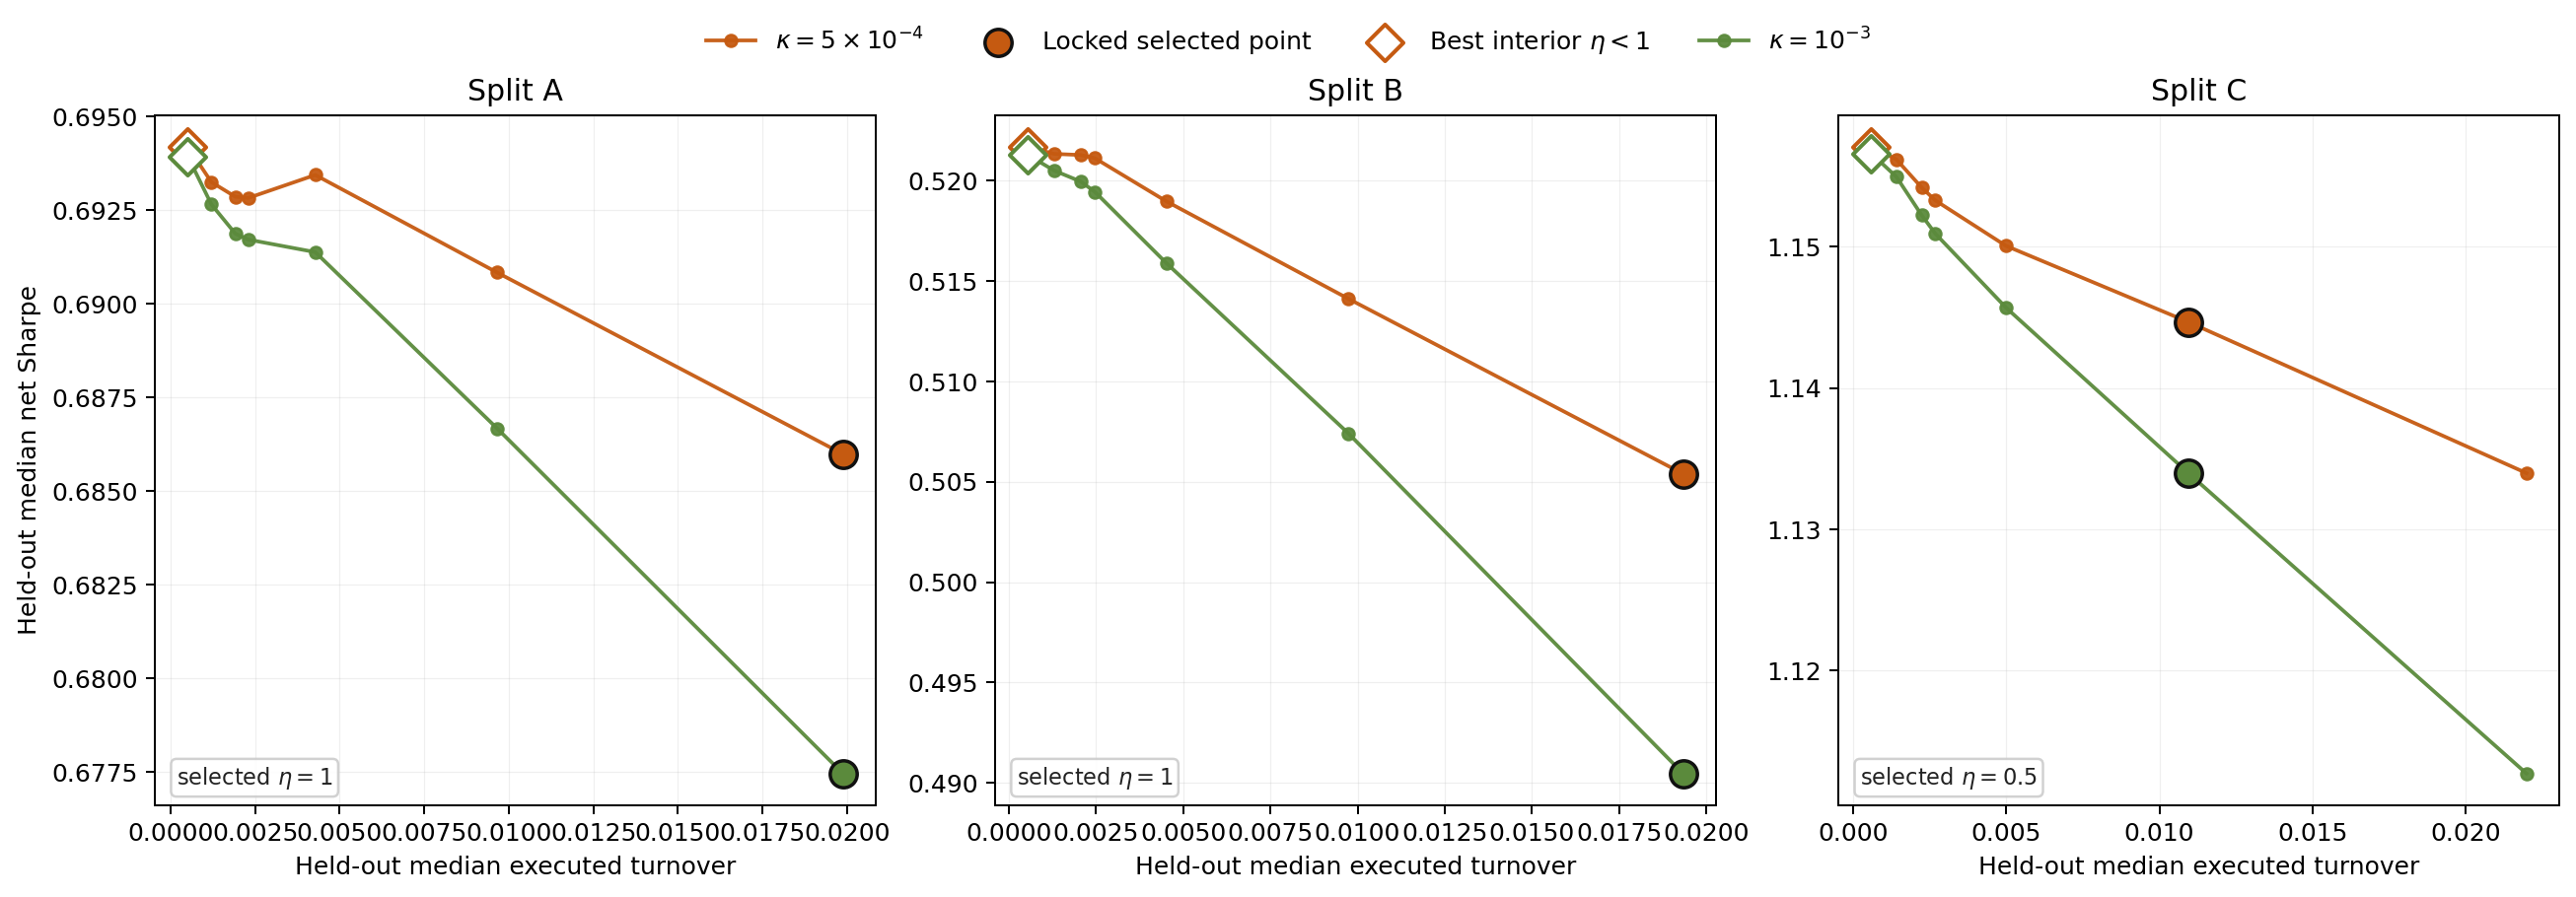
\includegraphics[width=0.92\textwidth]{fig_rolling_frontier_robustness.png}
\caption{Held-out positive-cost frontiers across the three rolling windows. Each panel shows the seed-median held-out net Sharpe versus seed-median executed turnover for $\kappa\in\{5\times10^{-4},10^{-3}\}$ over the fixed $\eta$ grid. Filled black-edged markers denote the locked validation-selected operating point for that split; hollow diamonds denote the best interior held-out point $\eta<1$, shown only as a post-selection diagnostic. Split C both selects and benefits from an interior point, whereas Splits A and B still exhibit interior frontiers even though the conservative selector remains at $\eta=1.0$.}
\label{fig:rollingfrontier}
\end{figure*}

\subsection{Denser friction grid: the frontier steepens as \texorpdfstring{$\kappa$}{kappa} grows}
We next densify the friction axis on the canonical split by adding $\kappa\in\{2\times10^{-4},2\times10^{-3}\}$ while keeping the frozen policy, the $\eta$ grid, and the validation-first protocol unchanged. This expansion is intentionally diagnostic: it does not retrain any policy and it does not replace the main selected-point result. Two findings are useful. First, the global validation selector remains stable. When positive costs are expanded to $\{2\times10^{-4},5\times10^{-4},10^{-3},2\times10^{-3}\}$, the same locked rule still selects $\eta=0.5$. Relative to immediate execution, that global selected operating point improves paired median net Sharpe by $+0.0041$, $+0.0105$, $+0.0213$, and $+0.0409$ as $\kappa$ increases across those four positive-cost regimes, while reducing median executed turnover by $0.01105$ in each row.

Second, the full held-out frontier becomes progressively more favorable to interior execution rates as friction grows. Using the best interior point only as a post-selection diagnostic, the paired median net-Sharpe gain versus $\eta=1.0$ rises monotonically from $+0.0113$ at $\kappa=2\times10^{-4}$ to $+0.0230$ at $\kappa=5\times10^{-4}$, $+0.0424$ at $\kappa=10^{-3}$, and $+0.0761$ at $\kappa=2\times10^{-3}$; the corresponding reduction in median executed turnover is essentially constant at about $0.02143$ because the comparison is always against the same immediate-execution baseline. A per-$\kappa$ diagnostic selector tells the same story from the other direction: it remains at $\eta=1.0$ for $\kappa=2\times10^{-4}$ and $5\times10^{-4}$, moves to $\eta=0.5$ at $\kappa=10^{-3}$, and tightens further to $\eta=0.2$ at $\kappa=2\times10^{-3}$. The friction-grid expansion therefore supports a simple interpretation: the execution frontier is not only real, but increasingly consequential as proportional trading frictions rise. Figure~\ref{fig:kappacurve} summarizes this tightening pattern across the dense friction grid.

\begin{figure*}[t]
\centering
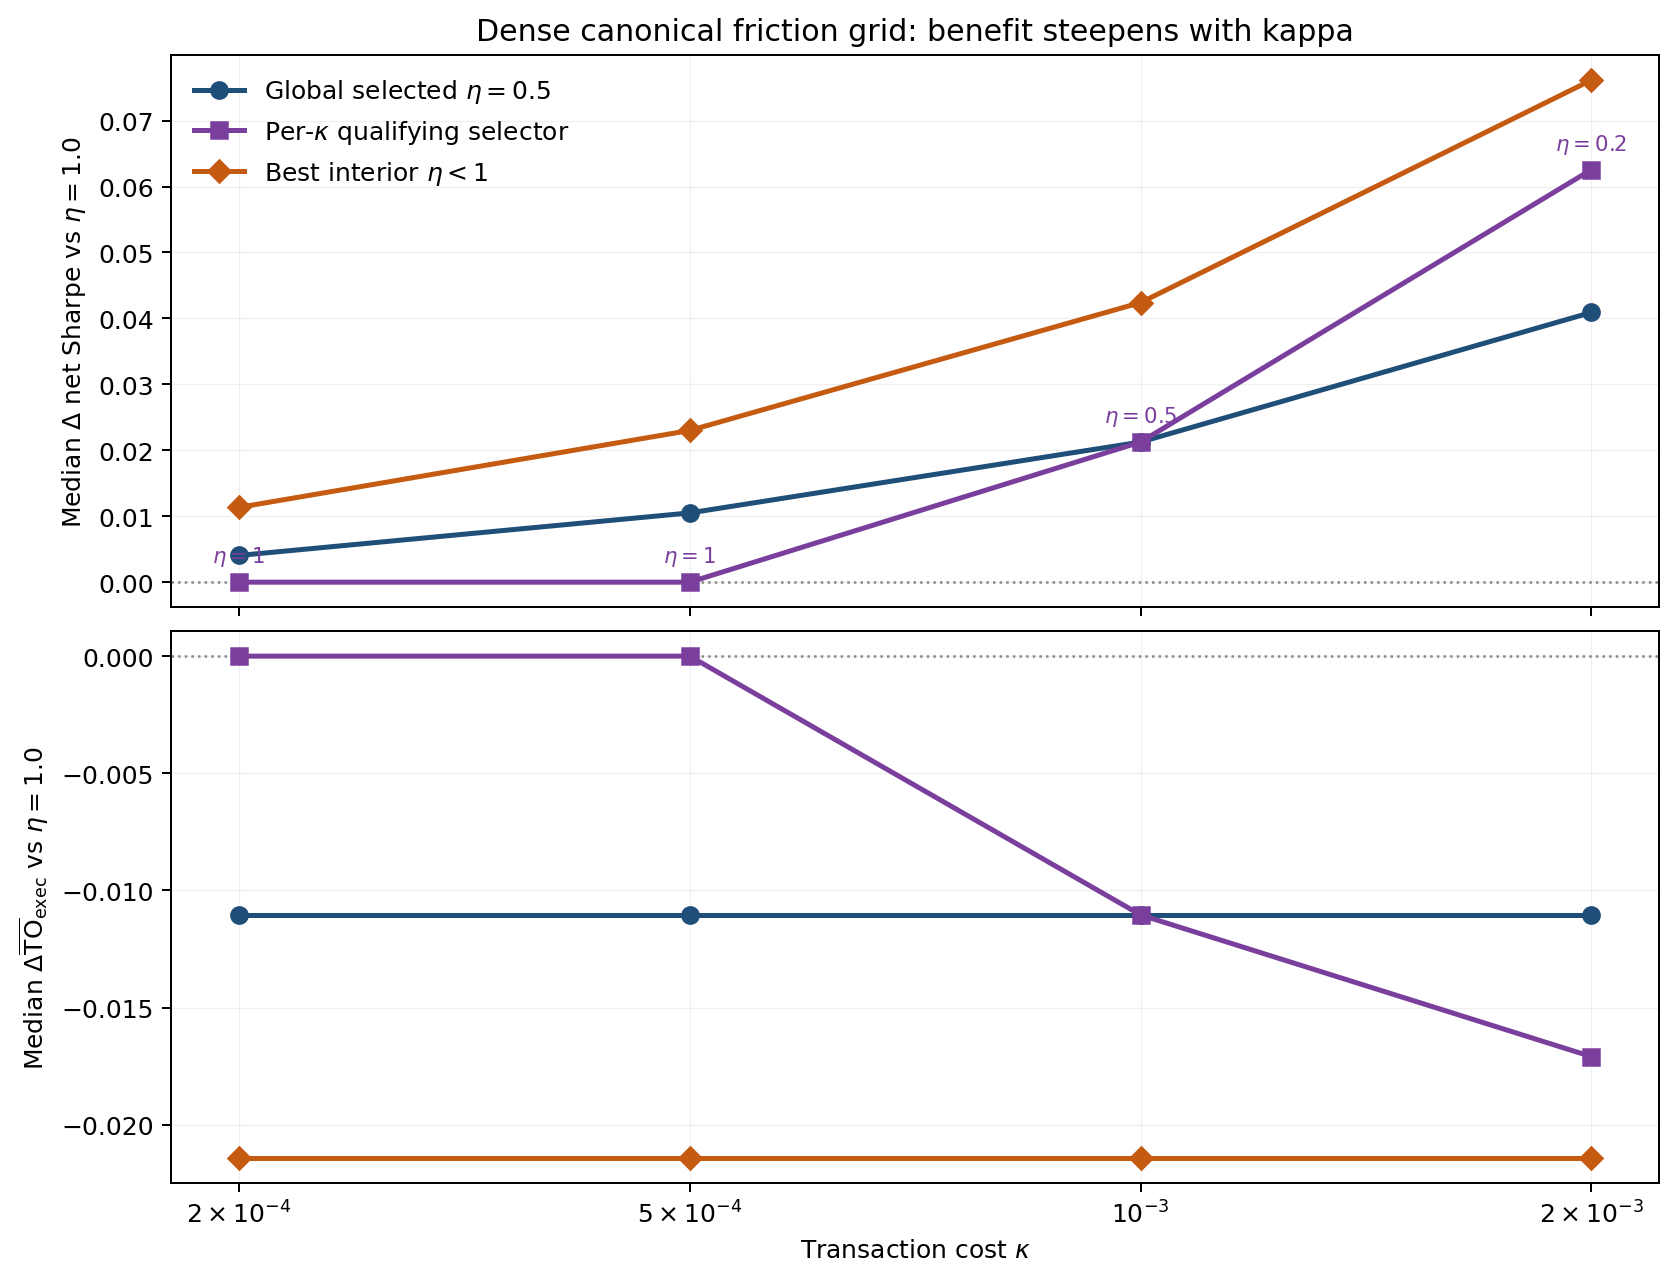
\includegraphics[width=0.80\textwidth]{fig_kappa_benefit_curve.png}
\caption{Dense canonical friction-grid benefit curve relative to immediate execution $\eta=1.0$. The top panel plots paired median $\Delta$ net Sharpe and the bottom panel plots paired median $\Delta\overline{\TOexec}$ on the held-out 2024--2025 split as $\kappa$ increases from $2\times10^{-4}$ to $2\times10^{-3}$. The blue line is the global validation-selected operating point $\eta=0.5$, the purple line is the per-$\kappa$ qualifying selector, and the orange line is the best interior held-out point $\eta<1$ shown only as a diagnostic. The per-$\kappa$ selector annotations show how the conservative operating point moves inward only once frictions become large enough, while the best-interior Sharpe gain steepens monotonically with $\kappa$.}
\label{fig:kappacurve}
\end{figure*}

\FloatBarrier
\subsection{Adaptive \texorpdfstring{$\eta_t$}{eta-t} schedules are out of scope}
Adaptive schedules are intentionally left out of the present version. The goal of this paper is to isolate the execution effect under a single frozen control model; adding rule-based $\eta_t$ schedules would mix execution design with schedule-selection effects. We therefore treat adaptive execution as future work and use the fixed-$\eta$ frontier as the main empirical object.

% ============================================================
\section{Discussion}
\paragraph{Interpretation: realized-path stabilization, not alpha creation.}
The central empirical result is not that a different prediction model has been learned, but that the same learned target path can be implemented in a more cost-aligned way under frictions. On the canonical 2024--2025 split, moving from immediate execution to the validation-selected interior operating point $\eta=0.5$ roughly halves median executed turnover and improves net Sharpe in the positive-cost regimes, while the corresponding gross-Sharpe change is slightly negative. The resulting interpretation is therefore narrow and mechanistic: under a fixed learned policy, execution-aware control improves risk-adjusted performance primarily through lower realized turnover and lower realized cost, not through additional predictive alpha.

\paragraph{When and why does execution help most?}
The evidence also clarifies when execution control matters most. First, its gains are concentrated in positive-cost regimes: on the canonical split, paired median net-Sharpe improvements are $+0.0105$ at $\kappa=5\times10^{-4}$ and $+0.0213$ at $\kappa=10^{-3}$, whereas the $\kappa=0$ result is negligible. Second, the selected interior operating point produces a substantial reduction in executed turnover while maintaining only modest target--executed mismatch. Third, on the denser canonical friction grid, the best interior held-out gain steepens monotonically with $\kappa$, indicating that the execution frontier becomes more consequential as frictions rise. Taken together, these patterns support a friction-sensitive stabilization view rather than a broad claim that smaller $\eta$ is universally better.

\paragraph{Rolling-window diagnostic.}
The rolling-window diagnostic should be read carefully. It does not show that one conservative validation-selected operating point transfers unchanged across windows. In two additional windows, the locked selector remained at $\eta=1.0$ because immediate execution stayed sufficiently close to the split-wise validation best. What persists more robustly is not selected-point transfer, but frontier existence: across all three windows, the positive-cost held-out frontier still contains interior execution rates that improve net Sharpe while lowering executed turnover relative to $\eta=1.0$. The rolling-window result therefore acts less as a broad robustness win than as a boundary condition on when conservative validation selection activates smoothing.

\paragraph{Matched heuristics as context only.}
The matched heuristic baselines provide only secondary context. Under aligned executed-path accounting, the selected operating point is competitive against several higher-churn comparators such as inverse-volatility risk parity and minimum-variance, mixed against daily-rebalanced equal weight and long-only mean-variance, and weaker than buy-and-hold equal weight on this window. These results help locate the empirical scale of the effect, but they do not define the paper's main claim, which remains the internal frozen-policy execution comparison.

\paragraph{Limitations.}
The limitation structure mirrors the contribution structure. The paper contributes executed-path accounting, a fixed-$\eta$ execution frontier analysis, and a frozen-policy empirical study; correspondingly, the present evidence is bounded by the market abstraction used for accounting, the fixed-timescale design, and the absence of retraining comparisons.
\begin{itemize}[leftmargin=*,itemsep=1pt]
\item The executed-path accounting contribution is established under a daily close-to-close abstraction on a fixed 27-name large-cap U.S. equity snapshot with a no-cash long-only simplex. These choices make the accounting object transparent, but they also limit market realism and leave survivorship-related bias unresolved.
\item The execution-mapping contribution is established only for fixed $\eta$ schedules. Adaptive schedules and richer execution-control laws are intentionally excluded so that execution design is not confounded with schedule-selection effects.
\item The empirical contribution isolates execution under one frozen control model. Its strongest selected-point transfer result appears on the canonical split, while the rolling-window diagnostic shows that frontier existence is more robust than conservative selected-point transfer. Training-time alignment and retraining comparisons remain outside the scope of this version.
\item Secondary heuristic comparisons are reported under aligned accounting only as matched context. Comparator breadth is not a main contribution of this version, and broader classical comparisons are left to follow-on work.
\end{itemize}

% ============================================================
\section{Conclusion}
We formulate execution-aware portfolio reinforcement learning by separating target and executed portfolios and attaching both trading costs and primary evaluation to the realized executed path. Empirically, the paper is intentionally narrow: one trained policy is reused throughout, only the execution mapping varies over a fixed \emph{a priori} $\eta$ grid, $\eta$ is selected on validation only, and the test split is reserved for held-out evaluation.

On the canonical 2022--2025 split, the validation-selected operating point $\eta=0.5$ roughly halves median executed turnover and improves paired median net Sharpe in both positive-cost regimes, while the $\kappa=0$ evidence remains negligible. Across three rolling windows, the positive-cost held-out frontier remains interior even when conservative selected-point transfer does not persist. On a denser canonical friction grid, the same global selected operating point remains $\eta=0.5$, while the best interior held-out gain increases monotonically with friction. Mechanistically, these gains are explained by lower realized turnover and lower realized cost rather than by improved gross Sharpe.

The safe claim is therefore narrow. Under a fixed learned trading policy, cost-aligned execution control creates an interior positive-cost execution frontier whose gains are driven primarily by lower realized turnover and lower realized cost, while selected-point transfer remains window-sensitive. This is not a claim about retraining superiority, universal selected-point transfer across windows, broad dominance over classical portfolio strategies, or deployment-grade point-in-time backtesting. Future work should therefore focus on explicit training-time alignment comparisons, broader comparator studies, and adaptive execution schedules built on top of this locked frozen-policy protocol.

% ============================================================
\clearpage
\onecolumn
\appendix
\section{Reproducibility Checklist}
\label{app:repro}
\begin{itemize}[leftmargin=*,itemsep=1pt]
\item Paired-seed evaluation across all arms.
\item Per-run config archiving and command logging.
\item Environment signature files to detect drift.
\item Automated aggregation outputs (tables/figures) generated from stored traces.
\item Hard-locked core definitions: \eqref{eq:exec_update}--\eqref{eq:reward}.
\end{itemize}

\section{Data and Protocol Clarifications}
\label{app:data_protocol}
\subsection{Fixed universe, cache, and adjusted-close data}
The paper rebuild uses a cache-only paper-mode snapshot built from daily adjusted close prices retrieved via \texttt{yfinance}. Adjusted close is used so that stock splits and dividend adjustments are reflected in the return series rather than treated as spurious price jumps. The processed cache for the locked run is the fixed directory \texttt{data/processed\_u27}, and the frozen training config uses a fixed-list universe with 27 assets:

\begin{quote}
\small\ttfamily
AAPL, AMGN, AXP, BA, CAT, CRM, CSCO, CVX, DIS, GS, HD, HON, IBM, INTC, JNJ, JPM, KO, MCD, MMM, MRK, MSFT, NKE, PG, UNH, V, VZ, WMT
\end{quote}
This is a reproducible fixed 27-name snapshot, not a historical point-in-time constituent reconstruction. Legacy project naming may still contain ``Dow30'', but the locked paper rebuild uses the fixed 27-name universe listed above. Accordingly, the empirical protocol should be interpreted as a controlled benchmark study with survivorship-related limitations, not as a deployment-grade backtest free of constituent-selection bias.

\subsection{Decision timing and return interval}
The backtest uses a close-to-close convention. At decision time $t$:
\begin{enumerate}[leftmargin=*,itemsep=1pt]
\item the state $s_t$ is built only from information available up to close $t$,
\item the policy outputs the target portfolio $\wtgt_t$,
\item the execution controller forms the executed portfolio $\wexec_t$ via \eqref{eq:exec_update},
\item transaction cost is charged on executed turnover $\TOexec_t$ via \eqref{eq:cost_exec},
\item the realized return applied to the portfolio is the next-period close-to-close return over $(t,t+1]$.
\end{enumerate}
Thus the paper uses the convention ``decide at close $t$, then hold $\wexec_t$ over $(t,t+1]$.'' This ordering is important because both return realization and cost accounting are attached to the executed portfolio rather than to the raw target action.

\subsection{Frozen split and model-selection lock}
The locked rebuild materializes the experiment configuration before evaluation. The train, validation, and held-out test windows are frozen as 2010--2021, 2022--2023, and 2024--2025, respectively. Because the state uses 30-day rolling features, the realized validation/test traces begin on 2022-02-15 and 2024-02-14 inside those split boundaries. The selected signal snapshot is also frozen before validation and test evaluation; in the rebuilt run, the frozen signal list is \texttt{reversal\_5d} and \texttt{short\_term\_reversal}. The $\eta$ grid is fixed \emph{a priori}, validation selects one operating point, and the test window is then used only for final evaluation of that selected operating point and matched comparators. Internal forward checks for 2026 were used only for engineering sanity and are not included in the paper tables or in $\eta$ selection.

\subsection{Constraint set and omitted assets}
All experiments use a long-only, fully invested simplex. In particular, portfolio weights are constrained to be non-negative and to sum to one each period. The present study does not include an explicit cash asset, leverage, or short positions. This means that the execution controller studies the effect of partial adjustment within a risky-asset simplex only. The no-cash design is intentional for interpretability, but it also limits the strategy class and should be read as a scope restriction rather than as a claim about the best practical trading interface.

\subsection{Backtest scope limitations}
The protocol is designed to be reproducible and internally consistent, but its scope remains limited in several ways:
\begin{itemize}[leftmargin=*,itemsep=1pt]
\item fixed 27-name large-cap U.S. equity snapshot rather than point-in-time constituent reconstruction,
\item no explicit cash asset,
\item long-only fully invested simplex,
\item daily close-to-close execution abstraction rather than intraday microstructure modeling,
\item frozen-policy empirical scope rather than a full retraining comparison.
\end{itemize}
These limitations do not invalidate the execution-accounting contribution, but they do bound the external claims that should be made from the current experiments.

\section{Implementation Details}
\label{app:implementation_details}
\begin{itemize}[leftmargin=*,itemsep=1pt]
\item Data source and cache: daily adjusted close prices retrieved via \texttt{yfinance} are materialized once and then reused in cache-only paper mode for training and evaluation.
\item Universe treatment: the present paper uses a fixed 27-name snapshot rather than a point-in-time constituent reconstruction.
\item Timing convention: features at time $t$ use information available by close $t$, and realized returns are applied over the next close-to-close interval $(t,t+1]$.
\item Anti-lookahead: observations use rolling historical returns, contemporaneous volatility estimates, and previous executed weights only.
\end{itemize}

\section{Secondary Matched-Heuristic Context}
\label{app:secondary_heuristics}
Table~\ref{tab:selected_vs_external} is reported only as secondary context and is not part of the main identification strategy. Under the same effective held-out dates, the same transaction-cost definition $\kappaTC\cdot\TOexec$, the same annualization $\sqrt{252}$, and the same $r_f=0$ convention, the selected operating point is stronger than inverse-volatility risk parity and minimum-variance, mixed against daily-rebalanced equal weight and long-only mean-variance, and weaker than buy-and-hold equal weight on this window. The safe reading is therefore limited: matched heuristics show that the selected operating point can look competitive against several higher-churn comparators under aligned accounting, but these comparisons do not define the paper's main claim and do not change the frozen-policy interpretation of the internal execution frontier.

\begin{center}
\captionsetup{type=table}
\captionof{table}{Held-out test comparison between the validation-selected operating point $\eta=0.5$ and matched heuristic baselines on the effective held-out dates 2024-02-14 to 2025-12-31 within the 2024--2025 split. All quantities use the same executed-path accounting conventions.}
\label{tab:selected_vs_external}
\scriptsize
\begin{tabular}{@{}llrrrrr@{}}
\toprule
$\kappaTC$ & Baseline & Baseline Sharpe & $\Delta$Sharpe & Baseline CAGR & $\Delta$CAGR & $\Delta\overline{\TOexec}$ \\
\midrule
$0$ & Buy-and-hold EW & 1.1726 & -0.0172 & 0.1651 & -0.0001 & +0.01095 \\
$0$ & Daily-rebalanced EW & 1.1530 & +0.0024 & 0.1646 & +0.0004 & +0.00106 \\
$0$ & Inverse-vol RP & 1.0772 & +0.0782 & 0.1416 & +0.0234 & -0.02210 \\
$0$ & Minimum-variance & 1.0649 & +0.0905 & 0.1219 & +0.0431 & -0.04160 \\
$0$ & Mean-variance (long-only) & 1.2269 & -0.0716 & 0.1841 & -0.0190 & -0.08780 \\
$5\times10^{-4}$ & Buy-and-hold EW & 1.1726 & -0.0279 & 0.1651 & -0.0018 & +0.01095 \\
$5\times10^{-4}$ & Daily-rebalanced EW & 1.1441 & +0.0005 & 0.1632 & +0.0001 & +0.00106 \\
$5\times10^{-4}$ & Inverse-vol RP & 1.0453 & +0.0994 & 0.1369 & +0.0264 & -0.02210 \\
$5\times10^{-4}$ & Minimum-variance & 1.0064 & +0.1382 & 0.1145 & +0.0487 & -0.04160 \\
$5\times10^{-4}$ & Mean-variance (long-only) & 1.1420 & +0.0027 & 0.1694 & -0.0061 & -0.08780 \\
$10^{-3}$ & Buy-and-hold EW & 1.1726 & -0.0386 & 0.1651 & -0.0035 & +0.01095 \\
$10^{-3}$ & Daily-rebalanced EW & 1.1353 & -0.0013 & 0.1617 & -0.0002 & +0.00106 \\
$10^{-3}$ & Inverse-vol RP & 1.0133 & +0.1206 & 0.1321 & +0.0294 & -0.02210 \\
$10^{-3}$ & Minimum-variance & 0.9480 & +0.1860 & 0.1072 & +0.0544 & -0.04160 \\
$10^{-3}$ & Mean-variance (long-only) & 1.0570 & +0.0770 & 0.1550 & +0.0066 & -0.08780 \\
\bottomrule
\end{tabular}
\par\vspace{2pt}\raggedright\footnotesize{\textit{Note:} All heuristic rows use the same effective held-out dates 2024-02-14 to 2025-12-31 and the same executed-path accounting conventions. Positive $\Delta\overline{\TOexec}$ means the selected RL arm trades \emph{more} than the comparator; negative values mean it trades less.}
\end{center}

\section{Supplementary Figures}
\label{app:supp_figures}

\begin{center}
\captionsetup{type=figure}

\includegraphics[width=0.88\textwidth]{fig_seed_scatter.png}
\captionof{figure}{Seed-wise paired $\Delta$ net Sharpe on the effective held-out dates 2024-02-14 to 2025-12-31 for the validation-selected operating point $\eta=0.5$ relative to the immediate-execution baseline $\eta=1.0$. This figure visualizes the same held-out paired comparison reported in Table~\ref{tab:selected_vs_eta1}. Each point is one seed-wise difference $\mathrm{Sharpe}_{\eta=0.5}-\mathrm{Sharpe}_{\eta=1.0}$, and the dotted horizontal line marks zero. All 10 paired seeds are positive in the two positive-cost regimes, matching the $10/10$ seed-win result reported in Table~\ref{tab:selected_vs_eta1}, whereas the $\kappa=0$ panel mixes positive and negative deltas.}
\label{fig:seedscatter}
\end{center}

\begin{center}
\captionsetup{type=figure}

\includegraphics[width=0.92\textwidth]{fig_misalignment.png}
\captionof{figure}{Representative held-out trace for the validation-selected operating point on the effective held-out dates 2024-02-14 to 2025-12-31 within the 2024--2025 split at $\eta=0.5$, $\kappa=10^{-3}$, seed 2. The top panel shows executed net equity and hypothetical target net equity, where the target path is the immediate move to the target portfolio used only for diagnostics. The bottom panel shows cumulative executed and target turnover. The representative seed is the selected-arm run whose held-out net Sharpe is closest to the median selected-arm net Sharpe across the 10 paired seeds at $\kappa=10^{-3}$.}
\label{fig:misalign}
\end{center}

% ============================================================
\begin{thebibliography}{99}
\bibitem{markowitz1952}
H. Markowitz, ``Portfolio Selection,'' \emph{The Journal of Finance}, 1952.

\bibitem{merton1973}
R. C. Merton, ``An Intertemporal Capital Asset Pricing Model,'' \emph{Econometrica}, 1973.

\bibitem{bertsimas1998}
D. Bertsimas and A. W. Lo, ``Optimal Control of Execution Costs,'' \emph{Journal of Financial Markets}, 1998.

\bibitem{moody1998}
J. Moody and M. Saffell, ``Learning to Trade via Direct Reinforcement,'' \emph{IEEE Transactions on Neural Networks}, 1998.

\bibitem{jiang2017}
Z. Jiang, D. Xu, and J. Liang, ``A Deep Reinforcement Learning Framework for the Financial Portfolio Management Problem,'' \emph{CoRR}, abs/1706.10059, 2017.

\bibitem{nevmyvaka2006}
Y. Nevmyvaka, Y. Feng, and M. Kearns, ``Reinforcement Learning for Optimized Trade Execution,'' \emph{Proceedings of the 23rd International Conference on Machine Learning}, 2006.

\bibitem{ye2020}
Y. Ye, H. Pei, B. Wang, P.-Y. Chen, Y. Zhu, J. Xiao, and B. Li, ``Reinforcement-Learning Based Portfolio Management with Augmented Asset Movement Prediction States,'' \emph{Proceedings of the AAAI Conference on Artificial Intelligence}, 34(1):1112--1119, 2020.

\bibitem{lien2023}
Y.-H. Lien, Y.-K. Li, and Y.-S. Wang, ``Contrastive Learning and Reward Smoothing for Deep Portfolio Management,'' \emph{Proceedings of the Thirty-Second International Joint Conference on Artificial Intelligence (IJCAI-23)}, pp. 3966--3974, 2023.

\bibitem{lobo2007}
M. Lobo, M. Fazel, and S. Boyd, ``Portfolio Optimization with Linear and Fixed Transaction Costs,'' \emph{Annals of Operations Research}, 152(1):341--365, 2007.

\bibitem{li2014}
B. Li and S. C. H. Hoi, ``Online Portfolio Selection: A Survey,'' \emph{ACM Computing Surveys}, 2014.

\bibitem{garleanu2013}
N. G\^arleanu and L. H. Pedersen, ``Dynamic Trading with Predictable Returns and Transaction Costs,'' \emph{The Journal of Finance}, 68(6):2309--2340, 2013.

\bibitem{almgren2000}
R. Almgren and N. Chriss, ``Optimal Execution of Portfolio Transactions,'' \emph{Journal of Risk}, 3(2):5--39, 2000.

\bibitem{shen2020}
Q. Shen, Y. Li, H. Jiang, Z. Wang, and T. Zhao, ``Deep Reinforcement Learning with Robust and Smooth Policy,'' \emph{Proceedings of the 37th International Conference on Machine Learning}, \emph{PMLR} 119:8707--8718, 2020.

\bibitem{mysore2021}
S. Mysore, B. Mabsout, R. Mancuso, and K. Saenko, ``Regularizing Action Policies for Smooth Control with Reinforcement Learning,'' \emph{Proceedings of the IEEE International Conference on Robotics and Automation (ICRA)}, pp. 1810--1816, 2021.
\end{thebibliography}

\end{document}
